\section{Path Tracer}
\label{path_tracer}
This section presents a closer look at the general path tracing process and highlights key implementation details of the evaluated CPU path tracer.
\subsection{Pipeline}
\begin{figure}[H]
    \centering
    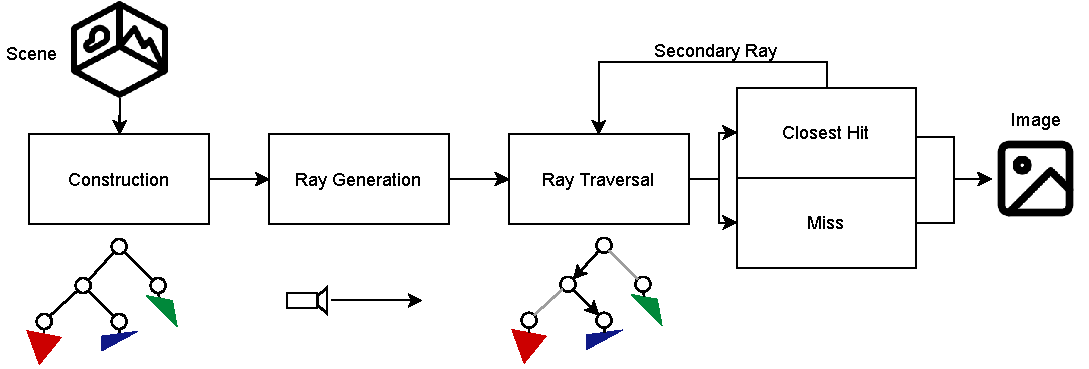
\includegraphics[width=400pt]{images/ray_trcing_pipeline.pdf}
    \caption{Visualization of path tracing process as a pipeline.}
    \label{fig:ray_pipeline}
\end{figure}
The graphics rendering process if often organized into a graphics pipeline\cite{sugerman09gramps}, so I generalized the path tracing process in a similar fashion (figure \ref{fig:ray_pipeline}). In the first stage of that pipeline the acceleration structure is created, which will be discussed further in section \ref{phr}. Given a static scene, this acceleration structure can be reused for multiple frames. Dynamic scenes require additional care though, as the acceleration structure either needs to be refit or rebuild on scene changes. The implemented uses a hybrid approach further elaborated in section \ref{phr_in_interactive}. The next stages are responsible for ray traversal and intersection testing. First, primary rays are generated from the camera's origin towards each pixel. Then, each ray has to traverse the acceleration structure to find the closest hit. Depending on whether or not this intersection has been found, either the closest hit shader, or the miss shader is called. Each shader can contribute to the color of the pixel, but only the closest hit shader spawns secondary rays. Note that my implementation uses implicit light sources instead of explicitly casting shadow rays. Secondary rays are fed back to the ray traversal stage and after reaching the maximum depth, the closest hit shader exits without creating any additional rays. The steps in these stages are embarrassingly parallel, however, because every ray is independent of the others, \acrshort{simd} instructions cannot be utilized. Consequently, each pixel is processed concurrently using multithreading.
\subsection{Intersection Tests}
A ray can be expressed using the parametric form 
\begin{equation} \label{eq:1}
    R(t)=O+t\textbf{d}
\end{equation}
where point $O$ defines the origin of the ray and vector \textbf{d} defines the direction along which the ray travels in a straight line. The path tracer supports two types of primitives, spheres and triangles. 
\subsubsection{Sphere}
Spheres are commonly used in ray tracing because of their simple and efficient intersection algorithm\cite{haines2019}. Given a sphere with center $C$ and radius $r$, all points $P$ at the surface of the sphere can be described by the equation:
\begin{equation} \label{eq:2}
    (P-G)\cdot(P-G)=r^2
\end{equation}
By substituting point $P$ in equation \ref{eq:2} by the equation of a ray (equation \ref{eq:1}) the intersection points between sphere and ray can be calculated. Simplifying the resulting equation leads to 
\[
    (\textbf{d}\cdot\textbf{d})t^2+2(\textbf{f}\cdot\textbf{d})t+\textbf{f}\cdot\textbf{f}-r^2 = at^2+b^t+c = 0
\]
which is a quadratic function. Consequently, it can be solved using 
\[
    t_{0,1}=\frac{-b\pm\sqrt{b^2-4ac}}{2a}
\]
with discriminant $\Delta=b^2-4ac$.
\begin{figure}[H]
    \centering
    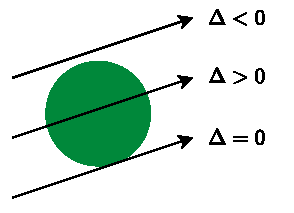
\includegraphics[width=150pt]{images/ray_sphere_intersection.pdf}
    \caption{Ray-sphere intersection test showing all three cases for discriminant $\Delta$.}
    \label{fig:sphere_intersec}
\end{figure}
As seen in figure \ref{fig:sphere_intersec}, if $\Delta<0$, the ray misses the sphere. If $\Delta=0$ the ray touches the sphere in one point and otherwise there are two values for $t$ that correspond to different intersection points. Inserting these $t$-values into equation \ref{eq:1} allows the calculation of intersection points $P_{0,1} = R(t_{1,2}) = O+t_{0,1}$\textbf{d}. The normal $n$ at a given intersection point is simply the vector from the spheres center $C$ to the intersection point $P$, i.e the normalized normal is calculated using $n=||P-C||$.

\subsubsection{Triangle}
Triangles have a long tradition in computer graphics, mainly because most geometry can be represented, or at least approximated, using them. Additionally, with 3 vertecies they can never be non-planar. While many ray-triangle intersection algorithms exist, the M{\"o}ller-Trumbore algorithm\cite{moeller97triangle} is still considered to be relatively fast and is often used as a comparison for other algorithms. Consequently, it is also used in this thesis. 

Using barycentric coordinates, a point $P$ on a triangle can be parameterized and expressed through two scalar values:
\[
    P(u,v) = (1-u-v)V_0 + uV_1 + vV_2
\]
where $V_0$, $V_1$ and $V_2$ are the vertices of given triangle and $(u,v)$ are the barycentric coordinates with $u\geq0$,  $v\geq0$ and $u+v\leq1$. Barycentric coordinates do not change when the triangle is transformed, which the M{\"o}ller-Trumbore algorithm exploits. Geometrically speaking, the algorithm translates the triangle to the origin and transforms it into a unit triangle in $y$ and $z$, with the ray direction aligned with $x$. This can be expressed as a system of linear equations:
\[
    \left[ \begin{array}{rrr}-\textbf{d}&(V_1-V_0)&(V_2-V_0)\end{array} \right]
    \left[ \begin{array}{r}t\\u\\v\end{array} \right] = O - V_0
\]
\begin{figure}[H]
    \centering
    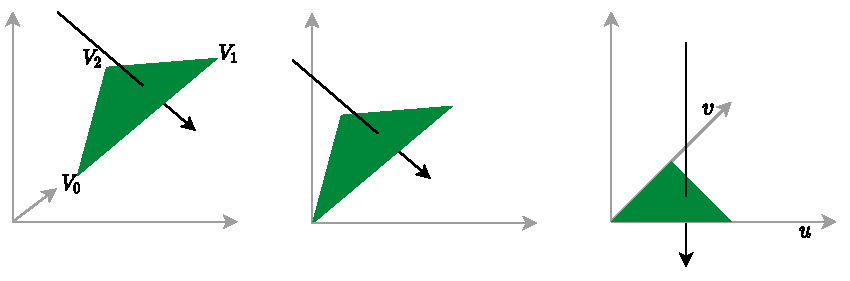
\includegraphics[width=400pt]{images/ray_triangle_intersec.pdf}
    \caption{Geometric representation of the transformations utilized in the M{\"o}ller-Trumbore algorithm.}
    \label{fig:triangle_intersec}
\end{figure}
Using Cramer's rule\cite{brunetti14cramersRule}, this system can be solved to obtain the distance $t$ from ray origin to intersection point and the corresponding barycentric coordinates $(u,v)$. Distance $t$ is again plugged into the ray equation to find the world coordinates of intersection point $P$ and the barycentric coordinates are used to interpolate the normal at $P$, given the vertex normals at $V_0$, $V_1$ and $V_2$.

\subsubsection{Axis-aligned bounding box}
Finally, bounding volume hierarchy traversal depends on a ray-bounding box intersection test. Axis-aligned bounding boxes are represented by the bounds $B^{min}$ and $B^{max}$, which define two planes for each dimension. The intersection distances $t$ between a given ray $R(t) = O+t\textbf{d}$ and a dimension $k$ can be computed fairly simple:
\[
    t^{min}_k = \frac{B_{k}^{min} - O_{k}}{\textbf{d}_{k}}
\]
\[
    t^{max}_k = \frac{B_{k}^{max} - O_{k}}{\textbf{d}_{k}}    
\]
Whether or not a ray intersects a box, can be determined by a few simple value comparisons, as seen in figure  \ref{fig:aabb_intersec}. The algorithm is optimized further by pre-computing sign and inverse direction for all rays and adding an early exit once it is clear the ray missed. 
\begin{figure}[H]
    \centering
    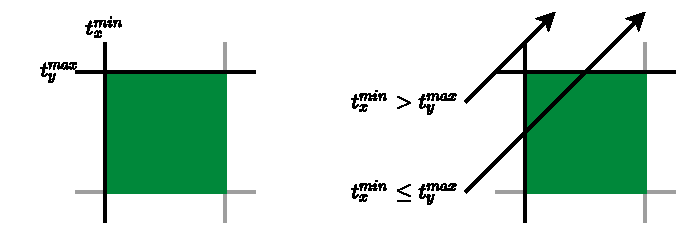
\includegraphics[width=400pt]{images/aabb_intersec.pdf}
    \caption{2D example of ray-AABB intersection. The top ray misses, while the bottom one hits the box.}
    \label{fig:aabb_intersec}
\end{figure}
\clearpage
\subsection{Materials}
Each primitive has an associated material. A material has an albedo specifying how reflective it is, i.e. how much color is contributed to the traced path, and an amount of emitted light. The scatter function differs between materials and is used to generate secondary rays. Note that it is also possible for materials to not scatter at all, which is used for light sources. 

Diffuse materials scatter rays in random directions. To achieve true Lambertian reflectance\cite{weik01lambert}, random points are picked on the surface of a unit sphere and added to the normal at intersection point. This results in a distribution of $cos(\Phi)$, where $\Phi$ is the angle from the normal. 

A smooth reflective material\cite{Greve2004ReflectionsAR} does not scatter rays in a random direction, so the resulting rays point purely in the reflection direction $\textbf{d}_r$ (figure \ref{fig:reflect_refract}):
\[
    \textbf{d}_r = \textbf{d} - 2\textbf{n}(\textbf{d}\cdot \textbf{n})
\]
where $\textbf{n}$ is the normalized normal at intersection point and $\textbf{d}$ is the direction of the incoming ray. For diffuse reflection a random vector is added to the reflected ray, similar to the above mentioned diffuse scattering.

Refractive materials\cite{Greve2004ReflectionsAR} utilize Snell's law to represent dielectrics like glass objects. Snell's law can be written as 
\[
    sin \theta' = \frac{\eta}{\eta'}sin \theta
\]
where $\theta$ and $\theta'$ are angles from the normal and $\eta$ and $\eta'$ are refractive indices. The refracted direction $\textbf{d}_t$, as shown in figure \ref{fig:reflect_refract}, can be split up into a parallel and a perpendicular part:
\[
    \textbf{d}_t=\textbf{d}_{\bot}+\textbf{d}_{\parallel}
\]
Solving for $\textbf{d}_{\parallel}'$ and $\textbf{d}_{\bot}'$ leads to:
\[
     \textbf{d}_{\bot}' = \frac{\eta}{\eta'}(\textbf{d}+(-\textbf{d}\cdot\textbf{n}) \textbf{n})
\]
\[
    \textbf{d}_{\parallel}' = - \sqrt{1-|\textbf{d}_{\bot}'|^{2}\textbf{n}}
\]
Adding both parts together, leads to the refracted direction $\textbf{d}_t$
\begin{figure}[H]
    \centering
    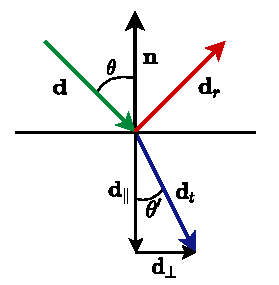
\includegraphics[width=200pt]{images/reflection_refraction.pdf}
    \caption{Figure showing how a ray's direction (green) is reflected (red) and refracted (blue).}
    \label{fig:reflect_refract}
\end{figure}
\subsection{Traversal}
\label{traversal}
To find the nearest intersection, bounding volume hierarchies are traversed in a top-down manner. Usually, this is done using a stack\cite{meister21survey} to store nodes that might contain an intersection. First, the root is pushed to the stack. While the stack is not empty, nodes are popped and checked for an intersection with their bounding box. In case the bounding volume is hit, either the nodes children are pushed onto the stack in the case of an interior node, or all primitives are tested when dealing with a leaf node. If no intersection with the bounding box is found or the distance to the intersection is bigger than previously found intersections, then the node can be discarded. Once the stack is empty, the closest intersection found is returned.

However, this method proved to be less efficient than using a recursive procedure as described in algorithm \ref{alg:traversal}. Given that the implementation is written for the CPU, this implicitly uses the CPU stack, which results in an equivalent execution as described above, albeit without explicitly managing a stack data structure.
\begin{algorithm}
\caption{Pseudocode of recursive BVH traversal}
\label{alg:traversal}
    \tcp{Start traversal at root}
    
    \SetKwFunction{FTraverse}{Traverse}
    \FTraverse{root}\;
    \;
    \SetKwProg{Fn}{Function}{:}{}
    \Fn{\FTraverse{node}}{
        \If{node.aabb not intersected} {
            \Return
        }
        \If{node is leaf} {
            \ForEach{primitive}{
                test for ray-primitive intersection
            }
        }
        \Else{
            \ForEach{child}{
                \FTraverse{child}
            }
        }
    }
\end{algorithm}
\cleardoublepage